% THIS IS AN EXAMPLE DOCUMENT FOR VLDB 2012
% based on ACM SIGPROC-SP.TEX VERSION 2.7
% Modified by  Gerald Weber <gerald@cs.auckland.ac.nz>
% Removed the requirement to include *bbl file in here. (AhmetSacan, Sep2012)
% Fixed the equation on page 3 to prevent line overflow. (AhmetSacan, Sep2012)

\documentclass{sig-alternative}
\usepackage{graphicx}
\usepackage{color}
\usepackage{balance}  % for  \balance command ON LAST PAGE  (only there!)
\usepackage{times}
\usepackage{url}
\usepackage{algorithm}
\usepackage[noend]{algorithmic}
\usepackage{subfigure}
\usepackage{xspace}
\usepackage[noend]{algorithmic}
\usepackage{enumerate}
\usepackage{multirow}
\usepackage{epstopdf}
\usepackage{cleveref}
\newcommand{\squishlist}{
   \begin{list}{$\bullet$}
    {
      \setlength{\itemsep}{0pt}
      \setlength{\parsep}{3pt}
      \setlength{\topsep}{3pt}
      \setlength{\partopsep}{0pt}
      \setlength{\leftmargin}{1.5em}
      \setlength{\labelwidth}{1em}
      \setlength{\labelsep}{0.5em} } }

\newcommand{\squishend}{
    \end{list}  }

\newcommand{\argmax}{\operatornamewithlimits{arg\ max}}

\newcommand{\eat}[1]{}
\newcommand{\todo}[1]{\textcolor{red}{{TODO: #1}}}
\newcommand{\add}[1]{\textcolor{red}{{ADD: #1}}}
\newcommand{\note}[1]{\textcolor{blue}{{#1}}}

\newtheorem{definition}{Definition}
\newtheorem{example}{Example}
\newtheorem{theorem}{Theorem}
\newtheorem{lemma}{Lemma}
\newtheorem{problem}{Problem}
\newtheorem{reduction}{Reduction}
\newcommand{\domain}{\mathcal{D}}
\newcommand{\attributes}{\mathcal{A}_D}
\newcommand{\hierarchy}{\mathcal{H}_D}
\newcommand{\attrhierarchy}{\mathcal{H}_A}
\newcommand{\workers}{\mathcal{W}}
\newcommand{\uentities}{\mathcal{E}}
\newcommand{\queryvector}{{\bf Q_S}}



\begin{document}

% ****************** TITLE ****************************************

\title{CrowdGather: Budgeted Entity Extraction over Hierarchies}

\numberofauthors{3} 

\author{
}

\maketitle

\begin{abstract}

\end{abstract}




\section{Introduction}
Combining human computation with traditional computer systems has been recently proven beneficial in a growing number of complex application domains, including entity deduplication~\cite{wang:2012}, crowdsourced database systems~\cite{franklin:2011, marcus:2011}, knowledge base completion~\cite{kondredi:2014, west:2014}, entity extraction and structured data collection~\cite{trushkowsky:2013, park:2014}. 

We focus on the problem of using the crowd to extract entities from {\em structured domains}, i.e., domains that can be fully described by a collection of predicates following a pre-specified structure (e.g., a hierarchy), while adhering to constraints on the monetary cost and latency of the extraction process. Recently, Trushkowsky et al.~\cite{trushkowsky:2013} studied the problem of {\em crowdsourced entity extraction} in the context of crowdsourced databases focusing on the completeness and cost of the result for a specific enumeration query, where each query can be viewed as a single point of the entity domain. 
Often, however, applications require extracting entities over multiple domain points at the same time raising several challenges. Next, we use examples from two real-world scenarios to illustrate these challenges. 

%How crowd-sourcing can be used to enumerate entities. 

%Reasons why ``Getting it all" will not work

%Reasons why Hidden DBs approaches do not work

\subsection{Challenges}
\ \\Challeges
\begin{enumerate}
\item Limited budget - exploiting known hierarchies of entities to maximize extracted entities.
\item Extract the tail of the popularity distribution.
\item Estimating the unseen (i.e., how many new entities will we get with an extra query).
\item Dependent sampling in single and multiple hierarchies.
\end{enumerate}

The first scenario is that of collecting listings, such as business, job or event listings.

Challenges to discuss:
\begin{enumerate}
\item Show how one can guide workers to different points of the domain. Ideally, example to show that with the same number of queries we get more data.
\item Given a budget how to select which points of the domain to focus on.
\end{enumerate}

The second scenario is that of 


\subsection{Contribution}
\ \\Contributions
\begin{enumerate}
\item Introduce problem of budgeted entity enumeration.
\item How to exploit hierarchies to maximize/diversify the set of extracted entities under a budget constraint. Prove complexity of the problem. 
\item Estimators for calculating the number of new entities per query.
\item Estimators for dependent nodes, single and multiple hierarchies.
\item Heuristics, UCB style algorithms, with guarantees for independent nodes.
\item Experimental evaluation \textcolor{blue}{(NOTE: we need to think of baselines)}.
\end{enumerate}



\section{An Overview}
In this section we first review the problem of {\em crowdsourced entity extraction} and introduce a {\em budgeted} version of the basic problem. Then, we formally define the problem of {\em budgeted entity extraction over multiple hierarchies}, and finally, present an overview of our solution for the latter.

\subsection{Crowdsourced Entity Extraction}
%Present problem of crowdsourced entity enumeration. 
Let $\domain$ be a domain of entities that follows an open-world assumption, that is, incomplete or no information is available about which entities are contained in $\domain$. We assume knowledge of a set of discrete attributes $\attributes = \{A_1, A_2, \dots, A_d\}$ characterizing $\domain$. Let $dom(A_i)$ denote the domain of each attribute $A_i  \in \attributes$. Then, $\domain$ is the Cartesian product of $dom(A_1), \dots, dom(A_d)$. In the reminder of the paper we will refer to each element of the Cartesian product as a {\em point} in $\domain$, i.e., a point is a possible combination of values of all dimensions. We will also refer to a collection of points for which only a subset of attributes shares the same value as a {\em slice} of $\domain$. For example all points for which attribute $A_1 = x$ but all other attributes may take any value constitute a slice. 

The basic version of {\em crowdsourced entity extraction}~\cite{trushkowsky:2013} seeks to enumerate entities that belong in a single slice $\domain_P$ of $\domain$, specified by a set of predicates $P$ over a subset of attributes in $\attributes$. For example, consider the entity domain $\domain$ to be that of all ``Concerts" and the attributes describing the entities in $\domain$ to be $\attributes = \{$``Band Name", ``Location", ``Music Genre"$\}$. An instance of crowdsourced entity extraction corresponds to listing concerts with LOCATION = ``Boston, MA" and GENRE = ``Rock". 

We assume three different types of crowdsourced queries for answering an entity extraction problem as the one described above. The first type corresponds to {\em single entity queries} where workers are required to provide ``one more" entity that satisfies the query predicates. The second type of queries corresponds to {\em queries of  size k} where workers are asked to provide up to $k$ distinct entities. Finally, the last type corresponds to {\em exclude list queries}. Here,  workers are provided with $l$ entities that have already been extracted and are required to provide up to $k$ distinct entities under the constraint that none of them is included in the exclude list. It is easy to see that the last type of queries generalizes the previous two. Therefore, in the remainder of the paper, we will consider that all queries of the third type. To describe a query, we will use the notation $q(k,l)$ denoting a query of size $k$ accompanied with an exclude list of length $l$. 

Assuming an infinite pool of crowd workers,  one can extract entities satisfying a set of desired predicates by repeatedly asking workers queries with different configurations $q(k,l)$ across {\em multiple rounds}. However, in a typical crowdsourcing environment, tasks have different costs depending on their difficulty. Thus, crowdsourced queries of different difficulties should also exhibit different costs. Given a query $q(k,l)$, we assume that its cost is given by a function $c(\dot)$ with the following properties: (a) given an exclude list of fixed length $l$ then $c(q(k^{\prime},l)) \geq c(q(k,l)),  \forall k^{\prime} \geq k$, and (b) given a fixed query size $k$ then $c(q(k,l^{\prime})) \geq c(q(k,l)), \forall l^{\prime} \geq l$. 

The above naturally gives raise to a tradeoff between the total number of extracted entities and the total cost. Let $\pi$ denote a {\em querying policy}, that is, a chain of query configurations defining the crowdsourced queries issued at each round. Moreover, let $\uentities(\pi)$ be the total number of unique entities extracted following policy $\pi$ and $C(\pi)$ be the total cost of following querying policy $\pi$. Finally, we assume a monetary budget $\tau_c$ imposing a constraint on the total cost of a selected querying policy. We define the problem of budgeted crowdsourced entity extraction as follows:

\begin{definition}[Budgeted Entity Extraction]
Let $\domain$ be a given entity domain and $\tau_c$ a monetary budget on the total cost of issued queries. The Budgeted Entity Extraction problem seeks to find 
a querying policy $\pi^*$ that maximizes the number of unique entities extracted $\uentities(\pi^*)$ under the constraint $C(\pi^*) \leq \tau_c$.
\end{definition}

Measuring the effectiveness of different policies on extracting entities requires reasoning about the number of {\em new entities} returned by each query. In the remainder of the paper, we also refer to the number of new entities extracted by a query as the {\em return of the query}. The exact number of new entities returned by each query is unknown before issuing the query and thus one needs to estimated it using the expected number of new entities returned by a query $q(k,l)$. In their recent work, Trushkowsky et al.~\cite{trushkowsky:2013} showed how techniques from the species estimation literature can be used to estimate the new entities returned by queries of the form $q(1,0)$. Furthermore, the authors propose a {\em pay-as-you-go} scheme where one repeatedly issues $q(1,0)$ queries to the crowd until the {\em marginal gain}, i.e., the difference between the new extracted entities and the querying cost, drops below a desired threshold. However, the proposed scheme is agnostic to budget constraints as it does not enforces them explicitly. 


%\subsection{Budgeted Entity Extraction}
%
%We assume a monetary budget imposing a limitation on the total number of queries that can be issued to workers. Let $\mathcal{P}(\domain)$ denote a the possible slices of the domain $\domain$. Moreover, let $S \subseteq \mathcal{P}(\domain)$ be a subset of selected slices from $\mathcal{P}(\domain)$, and $\queryvector$ a vector containing the number of queries issued to workers for each element in $S$.  We denote with $\uentities(\queryvector)$ the total number of  unique entities extracted from the queries in $\queryvector$ and $C(\queryvector)$ the total cost  of the queries in $\queryvector$. We define the problem of budgeted crowdsourced entity extraction as follows:
%
%\begin{definition}[Budgeted Entity Extraction]
%Let $\domain$ be an entity domain, $\beta_c$ be a monetary budget on the total cost of issued queries. The Budgeted Entity Extraction problem seeks to find a subset $S \subseteq \mathcal{P}(\domain)$ and the corresponding query vector $\queryvector$ that maximizes the number of unique entities extracted  $\uentities(\queryvector)$ under the constraint $C(\queryvector) \leq \beta_c$.
%\end{definition}


%Using the technique proposed by Trushkowsky et al.~\cite{trushkowsky:2013} one can: (a) either iterate over all the points in $\domain$ or (b) consider $\domain$ as a single slice until the budget is exhausted  However, these two extreme approaches come with obvious limitations.
%
%The limitations of the first approach are rather obvious. First, the number of points in $\domain$ is exponentially large with respect to the number of attributes specifying the domain, and hence, for domains with a large number of attributes iterating over all points can be prohibitive given a budget constraint. Second, there might exist a large number of sparse or non-populated points in $\domain$.  
%
%To understand the limitations of the second approach,  we point out that crowdsourced entity extraction can be viewed as being equivalent to sampling items from a population with an unknown {\em popularity distribution}. The popularity distribution quantifies the probability of observing an item in a random sample from the underlying population. The efficiency of crowdsourced entity extraction is heavily affected by the popularity distribution characterizing the underlying domain~\cite{trushkowsky:2013}. Under skewed distributions one needs to issue a large number of queries to workers to obtain a sufficient coverage of the underlying entities. In cases where the domain contains a large number of entities, the cost of the queries might be prohibitive under the given budget. Moreover, due to the skew of the popularity distribution one may not be able to extract entities from slices of the domain $\domain$, whose entities belong in the tail of the distribution. Next, we focus on hierarchical domains and discuss how one can exploit their structure when solving the problem of crowdsourced budgeted entity extraction. 

\subsection{Extracting Entities over Hierarchies}
Next, we focus on structured domains where each attribute in $\attributes$ are hierarchically organized. For example, we consider the domain of  ``Concerts", where the attributes describing the underlying entities are $\attributes = \{$``Band Name", ``Location", ``Music Genre"$\}$. It is easy to see that the values for the attribute LOCATION, as well as the values for the attribute MUSIC GENRE are hierarchically organized. For example, location can simply refers to a country or a state in a country or even a city. When multiple hierarchies describe the entity domain, we consider a {\em unified hierarchy} corresponding to a lattice formed by taking the crossproduct of all available hierarchies. We denote this crossproduct as $\hierarchy$. 

Each node in $\hierarchy$ represents a slice of the data domain. Again, we assume a querying model as the one described before, however, we assume that queries can be issued at the level of nodes in $\hierarchy$. The basic definition of budgeted entity extraction can be extended for hierarchical domains as follows:
\begin{definition}[Hierarchical Entity Extraction]
Let $\domain$ be a hierarchical entity domain, described by a lattice $\hierarchy$, $\beta_c$ be a monetary budget on the total cost of issued queries. The Budgeted Hierarchical Entity Extraction problem seeks to find querying policy $\pi_S^*$ over a subset of nodes $S \subseteq \hierarchy$ that maximizes the number of unique entities extracted  $\uentities(\pi_S^*)$ under the constraint $C(\pi_S^*) \leq \tau_c$.
\end{definition}

Notice that apart from determining the right policy over the possible query configurations $q(k,l)$ we are also required to detect the optimal subset of nodes in $\hierarchy$ to be queried so that the total number of extracted entities is maximized under the given budget constraint. Clearly the problem of budgeted hierarchical entity extraction is a generalization of the first problem. However, the problem becomes more challenging as the number of nodes in $\hierarchy$ is exponential with respect to the number of attributes characterizing the domain under consideration. Moreover, queries across different nodes in $\hierarchy$ are not independent, hence, one needs to be able to updates the estimated return for a specific node in $\hierarchy$ considering indirect information obtained from querying nodes related to it.

%\ \\ \textbf{Single Hierarchy:}
%
%\ \\ \textbf{Multiple Hierarchies:}
%
%\ \\(1) Describe how domain changes when query nodes are connected via hierarchies. Present example. 
%
%\ \\(2) Discuss why cost may increase as we query nodes lower in the hierarchy (i.e., more specialized queries). Cost is a function of both monetary cost and latency.
%
%\ \\(3) Present optimization problem with hierarchies.

\subsection{Solution Overview}
\label{sec:overview}
We present an overview of our proposed framework for solving the problem of budgeted hierarchical entity extraction. We assume a large entity domain $\domain$ described by a set of attributes $\attributes$ with each attribute $A \in \attributes$ following a known hierarchy $\attrhierarchy$. One challenge in large entity domains is detecting parts of the domain with a small number of entities and avoid spending a the given budget on those. A fundamental idea to our framework is maximizing the number of extracted entities under the given budget by exploiting the structure of each $\attrhierarchy$, i.e., (a) the domain partitioning imposed by $\attrhierarchy$  and (b) the overlap of the hierarchy nodes. 


The problem of budgeted entity extraction can be viewed as an online optimization problem over multiple rounds, where at each round we seek to find the best query-node combination so that the total number of extracted entities over all rounds is maximized. An overview of the proposed framework is shown in \Cref{fig:framework}.

\begin{figure}
	\begin{center}
	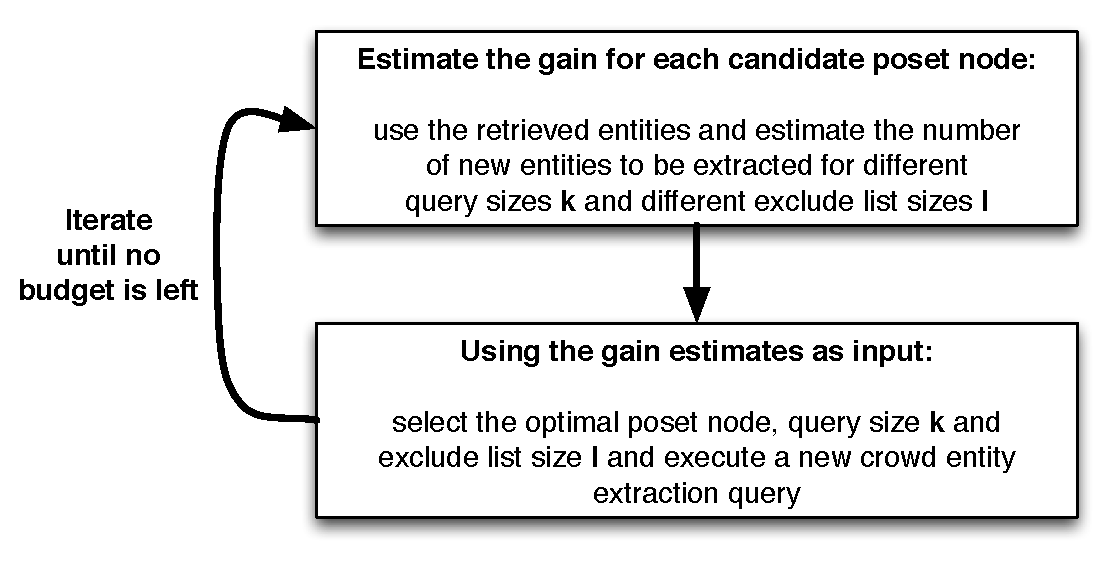
\includegraphics[clip,scale=0.5]{figs/framework.eps}
	\caption{Solution overview for budgeted entity extraction.}
	\label{fig:framework}
	\end{center}
\end{figure}

At a high-level, our solution consists of two major components. The first component is responsible for estimating the return obtained when an extra query $q(k,l)$ is issued at a certain node of $\hierarchy$. The second component takes as input the estimated returns for different nodes in the hierarchy and is responsible for finding the querying policy that will maximize the total return across all rounds under the specified budget constraints. We discuss the two components in \Cref{sec:estimation} and \Cref{sec:solution} respectively.  The following assumptions are made in the remainder of the paper:
\begin{itemize}
\item We assume that for each attribute $A \in \attributes$ the corresponding hierarchy $\attrhierarchy$ is known. 
\item We assume that after issuing a query we can associate each of the retrieved answers with all relevant nodes across all attribute hierarchies, i.e., a worker will provide all the attribute values describing a reported entity.
\end{itemize}

%At a high-level, our solution starts by selecting to query a node in $\hierarchy$ that maximizes the expected return, i.e., maximizes the difference between the {\em gain} from extracting entities and the {\em querying cost}. Then, depending on the retrieved entities, it selects one of the following actions: it (a) either continues querying the same node or (b) it selects to query a different node of similar level (i.e., different partitions of the entity domain) or (c) it progressively queries more specialized nodes originating from the current query node by traversing the hierarchy (\Cref{sec:solution}). This approach allows us to discover sparsely populated parts of the hierarchy in an online manner, and hence, limit the budget spent on them.
%
%The two main components of our approach are: (a) estimating the expected return for each available query node and (b) deciding which of the aforementioned actions to take. We discuss the two components in detail in \Cref{sec:estimation} and \Cref{sec:solution} respectively.  Finally, we make the following assumptions in the rest of the paper:
%\begin{itemize}
%\item We assume that the entire hierarchy describing the given entity domain is known. 
%\item We assume that after each query we can associate each of the retrieved answers with a leaf node in the hierarchy. In particular, we assume that a worker will provide all the attribute values describing a reported entity.
%\item Finally, we assume a fix type of queries that require each worker to provide us with a fixed number of unique entities per query. 
%\end{itemize}

%\ \\Give an overview of proposed solution
%\begin{enumerate}
%\item Input: Hierarchy, budget, cost per query.
%\item High-level description of online estimators. 
%\item Online optimization problem. 
%\end{enumerate}
%
%\ \\Clearly state and motivate the assumptions made throughout the paper
%\begin{enumerate}
%\item Entity hierarchies are known.
%\item Fixed query size (i.e., give me 5 more). Cost increases as we move to nodes lower in the hierarchy.
%\item After each query we can associate each of the answers with a leaf in the hierarchy. We assume full knowledge of all the attribute values of each entity.
%\end{enumerate}

\section{Estimating the Unseen Entities}
\label{sec:estimation}

%\textcolor{red}{Notes for this section:
%\squishlist
%\item Empirical estimates (extrapolation techniques) vs. chao based estimators
%\item Describe output of estimation component: Table N x C, where N corresponds to different nodes in the hierarchy, and C to different $q(k,l)$ query configurations
%\item Describe how to construct the exclude list, i.e., order items in decreasing order of appearance frequency and grab the top-$l$ items. 
%\item Came up with a new upper bound for the new number of items for different query sizes and different exclude list sizes. The upper bound combines extrapolation techniques with some of the tools used to derive the original Chao estimators. I need to test if the new upper bound is useful or not. 
%\item Bootstrapping to derive variance. 
%\item Consider if we should move away from purely empirical techniques and compare the new estimator with the standard Shen estimator. 
%\squishend}

The first component of our framework is responsible of estimating the number of new unique entities that will be extracted if a query $q(k,l)$ is issued at any node in $\hierarchy$, i.e., the return of $q(k,l)$ for a node $v \in \hierarchy$. We leverage techniques from the species estimation literature to solve the problem of estimating the return of a query $q(k,l)$ issued at any node in $\hierarchy$. We first show how the problem of estimating the return for queries of different sizes is equivalent to that of estimating the number of new species extracted by further sampling from an unknown population given a running sample~\cite{shen:2003} of retrieved items associated with a node $v$ in $\hierarchy$. We separate the available sample in two parts: (i) that extracted directly by querying $v$ and (ii) that obtained indirectly by querying other nodes in the hierarchy, and discuss how to exploit the information available for each of these two parts of the available sample. Then, we show how the proposed techniques can be extended for scenarios where an {\em exclude list} is provided. An exclude list can be formally defined as a set of observed entities that are provided to workers during query time and correspond to invalid answers that cannot be provided again. 

\subsection{Query Return and Species Estimation}
One of the most important problems in the species estimation literature is that of predicting the number of new species in further sampling. More precisely, we assume an unknown population of species and an initial sample from that population of size $n$. Given this setup, our goal is to predict the number of new species that will be discovered in a new sample of size $k$. Similarly during hierarchical crowdsourced entity extraction we have an unknown population of entities and our goal is to extract distinct entities from it. Different nodes in the hierarchy cover different parts of the population. In general this parts can be overlapping. The results of each query at a specific node can be viewed as a sample from the population corresponding to that node. Given a number of previously executed queries, we have a sample of observed entities for a specific node in $\hierarchy$. As in further sampling we want to estimate the number of new entities extracted from a new sample of size $k$. Moreover, we want to consider a given exclude list of size $l$. In this setup, we assume that information about the underlying population of a node under consideration has been retrieved by querying the node under consideration directly. However, we may also retrieve indirect information about a nodes population by querying other nodes in the hierarchy. Next, we discuss how to estimate the expected return for a node $v$ when considering the sampled items associated with $v$ that were retrieved by querying $v$ directly. In \Cref{sec:indirect} we discuss how one can exploit indirect information about the population of node $v$ to estimate the expected return of a query.

\subsection{Direct Information Estimators}
\subsubsection{Empty Answers}
If we have issued at least one query at a node $v \in \hierarchy$ and have received only empty answers, i.e., zero items, we assign its expected return to zero.

\subsubsection{Non-Empty Asnwers}
Next, we present an estimator for the return of a new query $q(k,l)$ that builds upon existing techniques from the species richness literature~\cite{shen:2003, hwang:2010}. 
Estimating the expected return of a query $q(k,l)$ for a specific node $v \in \hierarchy$ requires reasoning about the number of unseen entities in the population corresponding to $v$ and the conditional probability of discovering a new entity in an additional observation. Let $n$ denote the size of the running entity sample for node $v$ before issuing a new query, $S$ the total number of entities present in the world, and $D_n$ the number of distinct entities in the sample. Notice that $S$ is unknown. Finally, let $f_i$ denote the number of entities that appear $i$ times in the sample. Moreover, let $f_0$ denote the number of unseen entities from the underlying population and $C$ the sample coverage. The sample coverage denotes the conditional probability of finding an entity that has already been discovered in the sample if an additional observation were to be taken.  

First, we focus on estimating the number of unseen items in the underlying population $f_0$. We review an extrapolation based estimator proposed by Hwang and Shen~\cite{hwang:2010}. To derive this estimator Hwang and Shen make use of the generalized jackknife procedure for species richness estimation. Given two (biased) estimators of $S$, say $\hat{S}_1$ and $\hat{S}_2$, let $R$ be the ratio of their biases:
\begin{equation}
R = \frac{E(\hat{S}_1) - S}{E(\hat{S}_2) - S}
\end{equation}
By the generalized jackknife procedure, we can completely eliminate the estimating bias resulting from either $\hat{S}_1$ or $\hat{S}_2$ via
\begin{equation}
S = G(\hat{S}_1, \hat{S}_2) = \frac{\hat{S}_1 - R\hat{S}_2}{1 - R}
\label{eq:jknife}
\end{equation}
provided the ratio of biases is known. This is not true, and thus, we need to estimate $R$. 

We consider the following two biased estimators of $S$: $\hat{S_1} = D_n$ and $\hat{S}_2 = \sum_{j=1}^n D_{n-1}(j)/n = D_n - f_1/n$ where $D_{n-1}(j)$ is the number of species discovered with the $j$th observation removed from the original sample. Replacing these estimators in \Cref{eq:jknife} gives us:
\begin{equation}
S = D_n +\frac{R}{1-R}\frac{f_1}{n}
\end{equation}

Let $K = \frac{R}{1-R}$. From the Cauchy-Schwarz inequality we have:
\begin{equation}
K = \frac{\sum_{i=1}^S (1-p_i)^n}{\sum_{i=1}^S p_i(1-p_i)^{n-1}} \geq \frac{(n-1)f_1}{2f_2}
\end{equation}
This can be generalized to:
\begin{equation}
K=\frac{nf_0}{f_1} \geq \frac{(n-1)f_1}{2f_2} \geq \frac{(n-2)f_2}{3f_3} \geq \dots
\end{equation}
Let $g(i) = \frac{(n-i)f_i}{(i+1)f_{i+1}}$. From the above we have that the function $g(x)$ is a smooth monotone function for all $x \geq 0$. Moreover, let $y_i$ denote a realization of $g(i)$ mixed with a random error. Hwang and Shen how one can use an exponential regression model to estimate $K$. The proposed model corresponds to:
\begin{equation}
y_i = \beta_0\exp(\beta_1i^{\beta_2}) + \epsilon_i
\end{equation}
where $i = 1, \dots, n-1$, $\beta_0 > 0$, $\beta_1 < 0$, $\beta_2 >0$ and $\epsilon_i$ denotes random errors. It follows that $K = \beta_0$, and hence, $f_0$ can be approximated as $\hat{f}_0 = \frac{K\cdot f_1}{n}$.

Next, we focus on estimating the coverage $C$ of a running sample at node $v$. Let $n$ denote the size of the running sample, $f_1$ the number of singletons in the running sample. The coverage can be estimated by considering the Good-Turing estimator $\hat{C} = 1 - \frac{f_1}{n}$ for the existing retrieved sample 

Given the estimated number of unseen items and the coverage for the population corresponding to a node $v \in \hierarchy$ we can now estimate the number of new entities retrieved if we choose to issue a new query of size $k$ at $v$. For now we assume that no exclude list is specified. Then we will extend our approach to consider an exclude list of size $l$ together with a query of size $k$. 

\vspace{5pt}\noindent\textbf{Queries without an exclude list:}
We leverage techniques from the species estimation literature to estimate the expected number of new entities returned. Shen et al.~\cite{shen:2003}, derive an estimator for the number of new species $\hat{N}_{Shen}$ that would be found in an increased sample of size $k$. The approach assumes we have an estimate of the number of unobserved elements $\hat{f}_0$ and that the unobserved elements have equal relative abundances. For convenience we repeat the notation used above. Let $n$ as the size of the running sample, $f_1$ be the number of singletons in the running sample, $\hat{C}$ be the estimated coverage of the running sample and $\hat{f}_0$ be the estimated number of unseen species.  An estimate of the unique elements found in an increased sample of size $k$ is given by:
\begin{equation}
\label{eq:shen}
\hat{N}_{Shen} = \hat{f}_0 \left( 1 - \left(1 - \frac{1 - \hat{C}}{\hat{f}_0}\right)^k\right)
\end{equation}

\vspace{5pt}\noindent\textbf{Queries with an exclude list:}
Consider an exclude list of size $l$. As discussed before an exclude list is a set of items that correspond to invalid workers answers. Considering an exclude list for a query at a node $v \in \hierarchy$ corresponds to limiting our sampling to a restricted subset of the entity population corresponding to node $v$. In fact, we want to estimate the expected return of a query of size $k$ conditioning on the fact that the items in the exclude list will not be retrieved by any new sample. The latter corresponds to removing these items from the population under consideration. Thus, the estimates $\hat{f}_0$ and $\hat{C}$ should be updated before applying \Cref{eq:shen} to compute the expected return of a query of size $k$. This can be done by removing the items included in the exclude list from the running sample for node $v$, recomputing the entity counts $f_i$ and following the techniques presented above for computing the updated estimates for $\hat{f}_0$ and $\hat{C}$. This approach requires that the exclude list is known in advance. Next, we discuss how one can generate an exclude list of fixed size given a retrieved sample for a node $v \in \hierarchy$.


\subsubsection{Estimating the Expected Number of New Items Directly}
\label{sec:newestim}
We present a novel lower bound for the number of new entities for an increased query of some $m$. Let $n$ denote the existing sample size, $S$ the total number of entities present in the world, and $D_n$ the number of distinct entities in the sample. Finally, let $f_i$ denote the number of entities that appear $i$ times in the sample. To derive the new lower bound we make used of the generalized jackknife procedure for species richness estimation. Given two (biased) estimators of $S$, say $\hat{S}_1$ and $\hat{S}_2$, let $R$ be the ratio of their biases:
\begin{equation}
R = \frac{E(\hat{S}_1) - S}{E(\hat{S}_2) - S}
\end{equation}
By the generalized jackknife procedure, we can completely eliminate the estimating bias resulting from either $\hat{S}_1$ or $\hat{S}_2$ via
\begin{equation}
S = G(\hat{S}_1, \hat{S}_2) = \frac{\hat{S}_1 - R\hat{S}_2}{1 - R}
\label{eq:jknife}
\end{equation}
provided the ratio of biases is known. This is not true, and thus, we need to estimate $R$. 

We consider the following two biased estimators of $S$: $\hat{S_1} = D_n$ and $\hat{S}_2 = \sum_{j=1}^n D_{n-1}(j)/n = D_n - f_1/n$ where $D_{n-1}(j)$ is the number of species discovered with the $j$th observation removed from the original sample. Replacing these estimators in \Cref{eq:jknife} gives us:
\begin{equation}
S = D_n +\frac{R}{1-R}\frac{f_1}{n}
\end{equation}

Similarly, for a sample of increased size $n+m$ we have:
\begin{equation}
S = D_{n+m} +\frac{R^{\prime}}{1-R^{\prime}}\frac{f^{\prime}_1}{n+m}
\end{equation}
where $R^{\prime}$ is the ratio of the biases and $f^{\prime}_1$ the number of singleton entities for the increased sample.

Let $K = \frac{R}{1-R}$ and $K^{\prime} = \frac{R^{\prime}}{1-R^{\prime}}$. Taking the difference of the previous two equations we have:
\begin{equation}
D_{n+m} - D_{n} = K\frac{f_1}{n} - K^{\prime}\frac{f^{\prime}_1}{n+m}
\end{equation}

Therefore, we have:
\begin{equation}
\label{eq:new}
new = K\frac{f_1}{n} - K^{\prime}\frac{f^{\prime}_1}{n+m}
\end{equation}

We need to estimate $K$, $K^{\prime}$ and $f^{\prime}_1$. We start with $f^{\prime}_1$ denoting the number of singleton in the increased sample of size $n+m$. Notice, that $f^{\prime}_1$ is not known since we have not obtained the increased sample yet, so we need to express it in terms of $f_1$, i.e., the number of singletons, in the running sample of size $n$. We have:
\begin{equation}
f^{\prime}_1 = new + f_1 - f_1*\Pr[\mbox{in query of size m}]
\end{equation}
Following an approach similar to Shen et al.~\cite{shen:2003}, we have that the probability of a singleton appearing in a query of size $m$ is:
\begin{equation}
\Pr[\mbox{in query of size m}] = \sum_{k=0}^m(1-(1-\frac{1}{f_1})^k) {m \choose k}(1-p_1)^k p_1^{m-k}
\end{equation}
where $p_1$ denotes the probability that a singleton item in the sample of size $n$ will be selected in a future query. We estimate this probability using the corresponding Good-Turing estimator considering the running sample. We have:
\begin{equation}
p_1 = \hat{\theta}(1) = \frac{1}{n}2\frac{N_2}{N_1}
\end{equation} 
where $N_2$ is the number of entities that appear twice in the sample and $N_1$ is the number of singletons. 
Eventually we have that:
\begin{align}
f^{\prime}_1 &= new + f_1(1- \sum_{k=0}^m(1-(1-\frac{1}{f_1})^k) {m \choose k}(1-p_1)^k p_1^{m-k}) \nonumber \\
f^{\prime}_1 &= new + f_1(1- P)
\end{align}
Replacing the last equation in \Cref{eq:new} we have:
\begin{align}
&new = K\frac{f_1}{n} - K^{\prime}\frac{new + f_1(1- P)}{n+m} \nonumber \\
&new = K\frac{f_1}{n} - K^{\prime}\frac{new}{n+m} - K^{\prime}\frac{f_1(1- P)}{n+m} \nonumber \\
&new(1 + \frac{K^{\prime}}{n+m}) = K\frac{f_1}{n} - K^{\prime}\frac{f_1(1- P)}{n+m} \nonumber \\
&new = \frac{1}{(1 + \frac{K^{\prime}}{n+m})}(K\frac{f_1}{n} - K^{\prime}\frac{f_1(1- P)}{n+m}) \nonumber
\end{align}

Next, we discuss how one can estimate $K$ and $K_{\prime}$. To estimate $K$ we follow the extrapolation approach introduced by Hwang and Shen~\cite{hwang:2010}. Namely, from the Cauchy-Schwarz inequality we have that:
\begin{equation}
K = \frac{\sum_{i=1}^S (1-p_i)^n}{\sum_{i=1}^S p_i(1-p_i)^{n-1}} \geq \frac{(n-1)f_1}{2f_2}
\end{equation}
This can be generalized to:
\begin{equation}
K=\frac{nf_0}{f_1} \geq \frac{(n-1)f_1}{2f_2} \geq \frac{(n-2)f_2}{3f_3} \geq \dots
\end{equation}
Let $g(i) = \frac{(n-i)f_i}{(i+1)f_{i+1}}$. From the above we have that the function $g(x)$ is a smooth monotone function for all $x \geq 0$. Moreover, let $y_i$ denote a realization of $g(i)$ mixed with a random error. Hwang and Shen how one can use an exponential regression model to estimate $K$. The proposed model corresponds to:
\begin{equation}
y_i = \beta_0\exp(\beta_1i^{\beta_2}) + \epsilon_i
\end{equation}
where $i = 1, \dots, n-1$, $\beta_0 > 0$, $\beta_1 < 0$, $\beta_2 >0$ and $\epsilon_i$ denotes random errors. It follows that $K = \beta_0$. 

Finally, we show how one can estimate the value of $K_\prime$ for an increased sample of size $n+m$. First, we show that $K$ increases monotonically as the size of the running sample increases. Let $K(n) = \frac{\sum_{i=1}^S (1-p_i)^n}{\sum_{i=1}^S p_i(1-p_i)^{n-1}}$ be a function returning the value of $K$ for a sample of size $n$. We have the following lemma. 

\begin{lemma}
We have $K(n+m) \geq K(n), \forall n,m > 0$.
\end{lemma}
\begin{proof}
In the remainder of the proof we will denote $K(n+m)$ as $K^{\prime}$. By definition we have that $K = \frac{\sum_{i=1}^S (1-p_i)^n}{\sum_{i=1}^S p_i(1-p_i)^{n-1}}$ and $K^{\prime} = \frac{\sum_{i=1}^S (1-p_i)^{n+m}}{\sum_{i=1}^S p_i(1-p_i)^{n+m-1}}$. We want to show that:
{\small
\begin{align}
&\frac{\sum_{i=1}^S (1-p_i)^{n+m}}{\sum_{i=1}^S p_i(1-p_i)^{n+m-1}} \geq \frac{\sum_{i=1}^S (1-p_i)^n}{\sum_{i=1}^S p_i(1-p_i)^{n-1}} \nonumber \\
&\sum_{i=1}^S (1-p_i)^{n+m}\sum_{j=1}^S p_j(1-p_j)^{n-1} \geq \sum_{i=1}^S p_i(1-p_i)^{n+m-1}\sum_{j=1}^S (1-p_j)^n\nonumber \\
&\sum_{i,j:i\prec j}[(1-p_i)^{n+m}p_j(1-p_j)^{n-1} - p_i(1-p_i)^{n+m-1}(1-p_j)^n + \nonumber \\
& + (1-p_j)^{n+m}p_i(1-p_i)^{n-1} - p_j(1-p_j)^{n+m-1}(1-p_i)^n] \geq 0 \nonumber \\
&\sum_{i,j:i\prec j}[(1-p_i)^{n}(1-p_j)^{n-1}p_j((1-p_i)^{m} - (1-p_j)^{m})  + \nonumber \\
& - (1-p_j)^{n}p_i(1-p_i)^{n-1}((1-p_i)^{m} - (1-p_j)^{m}) \geq 0 \nonumber \\
&\sum_{i,j:i\prec j}[(1-p_i)^{n-1}(1-p_j)^{n-1}(p_j-p_i)((1-p_i)^{m} - (1-p_j)^{m}) \geq 0
\end{align}}

But the last inequality always holds since each term of the summation is positive. In particular, if $p_j \geq p_i$ then
also $1-p_i \geq 1-p_j$ and if $p_j \leq p_i$ then $1-p_i \leq 1-p_j$.
\end{proof}

We have that $K(n)$ is an increasing function of the sample size. Moreover, $K(n)$ has a decreasing slope. We model $K$ as a generalized logistic function of the form $f(x) = \frac{A}{1+exp(-G(x-D))}$. As we observe samples of different sizes for different queries we estimate $K$ as described above and therefore we observe different realizations of $f(\cdot)$. Thus, we can learn the parameters of $f$ and use it to estimate $K^{\prime}$.

\subsection{Indirect Information Estimators}
\label{sec:indirect}
\begin{figure*}[ht]
	\begin{center}
	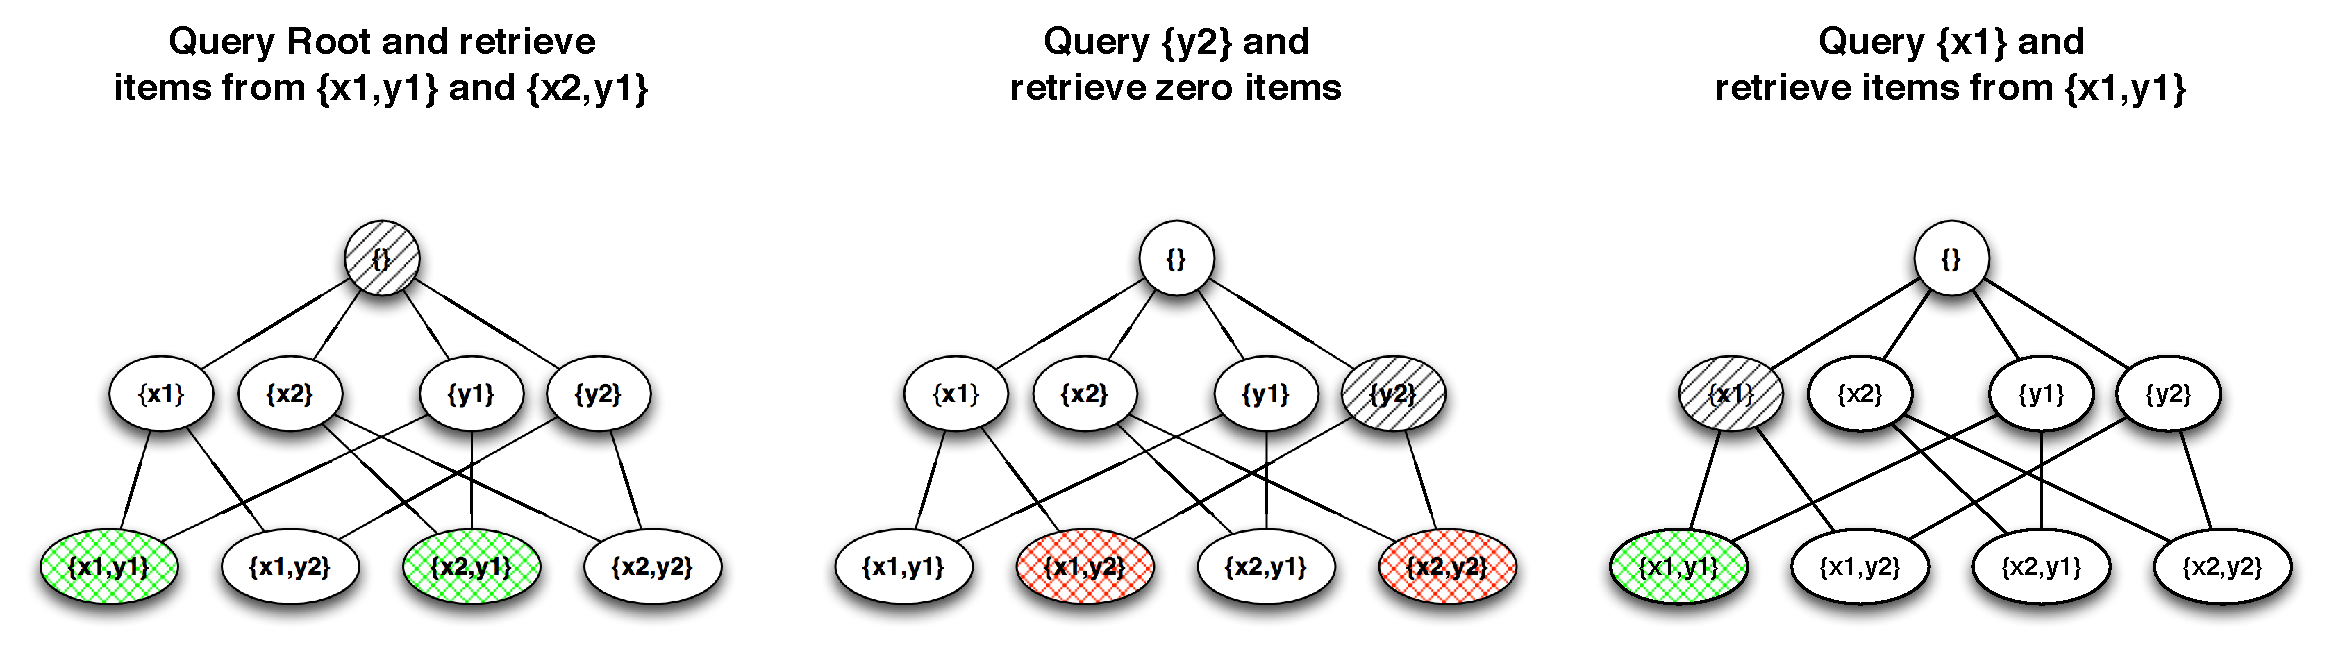
\includegraphics[clip,scale=0.4]{figs/examples.eps}
	\caption{Query examples on a two attribute lattice.}
	\label{fig:examples}
	\end{center}
\end{figure*}

Apart from directly querying a node in $\hierarchy$ and retrieving information about its underlying item population, we can also obtain information indirectly by querying other nodes in the hierarchy. Next, we identify four potential cases characterizing how information about the population of a node $v \in \hierarchy$ can be obtained indirectly. Given a node $v \in \hierarchy$ we identify the following cases:
\begin{enumerate}
\item We issue a query at an ancestor $u$ of $v$ and retrieve some items associated with $v$. 
\item We issue a query at an ancestor $u$ of $v$ and retrieve zero items associated with $v$ but some items associated with $u$.
\item We issue a query at an ancestor $u$ of $v$ and retrieve zero items associated $u$.
\item We issue a query at a non-ancestor node $u$ of $v$ and retrieve information about a descendant $l$ of  $v$. This information can be either that some items are associated with $l$ or that no items are associated with $l$.
\end{enumerate}

Examples of these cases are illustrated in \Cref{fig:examples}. \Cref{fig:examples} shows different query scenarios for a two attribute lattice. In the first figure, we receive some items for nodes $\{x1,y1\}$ and $\{x2,y1\}$ by querying the root of the lattice. This corresponds to case 1. Moreover, notice that no items were retrieved for nodes $\{x1,y2\}$ and $\{x2,y2\}$. This corresponds to case 2. In the second figure, we issue a query at node $\{y2\}$ and retrieve no items. This corresponds to case 3 for nodes $\{x1,y2\}$ and $\{x2,y2\}$ . Finally, in the last figure we issue a query at node $\{x1\}$ and retrieve some items for node $\{x1,y1\}$ and thus some items for node $\{y1\}$ but by querying its non-ancestor node $\{x1\}$. This corresponds to case 4 for node $\{y1\}$. Next, we discuss how one can reason about the available indirect information for each of the four cases provided above.

\subsubsection{Empty Answers from Ancestors}
When we issue a query at an ancestor $u$ of a node $v$ and receive not items associated with $v$ there are two potential cases as mentioned above. We either retrieved some items for other descendants of $u$ or received zero items for $u$ as well. In the first case, we do not have enough information to update our estimates for the expected return of a query $q(k,l)$ at node $v$. \textcolor{red}{the reason is the popularity distribution mixture but we need to explain this better}. Thus, we assume no information for the underlying population of $v$, i.e., the expected return is set to $k$. When we receive an empty answer for $u$ then we can safely update our estimate for $v$ to zero as well. 

\subsubsection{Non-Empty Answers from Ancestors}
When we issue a query at an ancestor of a node $v$ and retrieve a set of items associated with $v$ we consider the entire population of items associated with node $v$. Thus, we can consider this case as querying node $v$ directly but with a query of unknown size and exclude list. In this case, we can use the estimators for direct information presented before where we simply update the frequency counts consider the items retrieved by the new sample. Notice, that the size of the sample and the size of the exclude list used at the ancestor node does not affect the estimates for node $v$. \textcolor{red}{I think this holds for the case when no exclude list is used but I have a feeling this statement might not be correct when an exclude list is used, i.e., we may need to propagate the exclude list information from the parent to the child}.

\subsubsection{Information on Descendants Obtained by Non-Ancestor Nodes}
In this case only a subset of the population that corresponds to $v$ is used during sampling and this bias needs to be taken into account when estimating the expected return for $v$ when using this sample.

We propose the following approach to estimate the expected return in the presence of indirect information. Consider a node $v$ and a let $\mathcal{C}_v$ denote the immediate descendants, i.e., the children of $v$. Moreover, for each node $u \in \mathcal{C}_v$ let $p_u$ denote the probability of retrieving an item corresponding to $u$ when querying $v$ directly. We require that $\sum_{u \in \mathcal{C}_v} p_u = 1$. Given the probabilities $p_u$ we estimate the expected return of a query $q(k,l)$ at node $v$ as:
\begin{equation}
\label{eq:mixture}
r(v) = \sum_{u \in \mathcal{C}_v} p_u\cdot r(u)
\end{equation}
where $r(\cdot)$ denotes to the expected return of different nodes given that a $q(k,l)$ is issued at node $v$. 

\textcolor{red}{The things we need to do here: How do we estimate probabilities $p_u$. One approach might be to start from a uniform distribution and follow a frequentist's approach where we keep updating these probabilities based on how the answers of direct queries to $v$ are distributed across to its children. Notice that this can be done only for direct queries. How can we estimate $r(u)$ for any node $u$ by combining the information obtained by the directly sampled items and the indirectly sampled items. In particular we need a way to combine the biased regression based estimators corresponding to samples that considered the entire population and the estimator of \Cref{eq:mixture} that handles cases where the samples focused on subspaces of the population of $v$.}

\subsection{Constructing an Exclude List}
Intuitively, an exclude list should contain items that have high probability of appearing in a sample taken from the underlying population. According to the Good-Turing estimation technique the probability of an entity appearing to a new sample is correlated to the number of times that entity has been observed in the retrieved sample. In particular, we have that the probability for entity which were seen $r$ times is:

\begin{equation}
p_r = \frac{(r+1)S(N_{r+1})}{nS(N_r)}
\end{equation}
where $n$ is the total size of the retrieved sample, $N_r$ shows how many times the frequency $r$ occurs in the retrieved sample, and $S()$ is the smoothed or adjusted value of the frequency shown in parenthesis. One basic assumption of the Good-Turing estimation techniques is that items with the same frequency $r$ in the retrieved sample have the same probability $p_r$ of appearing in a new sample. 

\subsubsection{Deterministic Construction}
To construct an exclude list deterministically, we consider ordering of the retrieved items in decreasing order of their popularity and selecting the top-$l$ items to be included in a list of size $l$. It is easy to see that this approach restricts future queries to use an exclude list of size at least $l$ as items already included in the exclude list should always be included and if new items become frequent then the size of the exclude list should be extended so that it contains all frequent items. More precisely let $\mathcal{O}_n$ denote the ordering of retrieved items with respect to there popularity when the size of the retrieved sample is $n$, and $\mathcal{O}_m$ be the corresponding ordering when the size of the the retrieved sample is $m \leq n$. For both orderings assume an exclude list of size $l$. We require that  $\forall l,n,m$ with $l \leq n \leq m$ top-$l(\mathcal{O}_m)$ = top-$l(\mathcal{O}_n)$. 

\textcolor{red}{Last time we said that we need to increment the item count for its item in the exclude list by one. This is not correct. I think we should increment its count considering the average appearance frequency in the previous samples. I think this will mention the relative ordering requirement described above but we need to prove that.}
\subsubsection{Randomized Construction}
To construct a randomized list pick $l$ of the retrieved items uniformly at random. We argue that uniform sampling is necessary so that we are not biased against specific items from the already retrieved sample. \textcolor{red}{Not sure how we can justify this.}

\section{Cost Models for Entity Extraction Queries}

Cost models we should consider:
\begin{enumerate}
\item  Uniform cost, regardless of the point $v \in \hierarchy$ the query size and the exclude list size.
\item  Cost that increases proportionally to the distance of $v \in \hierarchy$ from the root. That is more specialized queries cost more.
\item  Extend previous cost to consider the size of the query and/or the size of the exclude list. The cost can increase exponentially with respect to these numbers. 
\end{enumerate}

\section{Solving Budgeted Entity Extraction}
\label{sec:solution}
Assume a hierarchy $\hierarchy$. The return of issuing queries at different nodes in $\hierarchy$ is unknown in advance. However with every new query we issue at a node of $\hierarchy$ we obtain more information about entities extracted from different nodes of $\hierarchy$. As discussed above, we can use this information to obtain more accurate estimated on the expected return of new queries for different nodes in $\hierarchy$. In the previous section we described how one can estimate the expected return for a node $v \in \hierarchy$ for a generalized query $q(k,l)$, given a retrieved sample while considering different values of $k$ and $l$. 

Given this setup one can consider the problem of {\em budgeted entity extraction} as an adaptive optimization problem where we simultaneously attempt to acquire new knowledge and also optimize our decisions on existing knowledge. Consider an algorithm $\mathcal{A}$ that attempts to solve this problem. Then it is natural to say that this algorithm proceeds in {\em rounds} and its goal is to maximize the overall return across all rounds. At each round $\mathcal{A}$ uses the existing information to choose the best action from a set of potential actions. For budgeted entity extraction, the set of potential actions an algorithm $\mathcal{A}$ can take at each round, corresponds to the set of all queries $q(k,l)$, for all valid values of $k$ and $l$, issued at the different node of $\hierarchy$. Next, we discuss how one can design such an algorithm $\mathcal{A}$ for solving the problem of budgeted entity extraction. Before presenting our proposed algorithm we list several challenges associated with this adaptive optimization problem.

\subsection{Challenges}
\begin{enumerate}
\item The first challenge is that the number of nodes in $\hierarchy$ is exponential with respect to the number of attributes $\attributes$ describing the domain of interest. Querying every possible node to estimate its expected return for different queries $q(k,l)$ is prohibitively expensive. In fact, it is natural to assume a budget that does not allow any algorithm to query all nodes in the hierarchy. However, we assume that keeping estimates for each of the nodes for which at least one entity has been retrieved is feasible. 
\item Balance exploration and exploitation.
\item Querying a specific node in the hierarchy provides indirect information for other nodes in the hierarchy. Our proposed technique is capable of exploiting these dependencies across nodes to obtain more accurate estimates. An example of such dependencies is that one should be able to reason about the variances of children considering the variances of parents. 
\item Given a fixed query size and a fixed exclude list size, the expected return of a new query for a node is a decreasing function.
\end{enumerate}
Next, we focus on each of these challenges.

\subsection{Balancing Exploration and Exploitation}

While issuing different queries $q(k,l)$ at different nodes of $\hierarchy$ we obtain a collection of entities that can be assigned to different nodes in $\hierarchy$. For each such node we can estimate the return of a new query $q(k,l)$ using the estimator presented in \Cref{sec:newestim}. However, this estimate is based on a rather small sample of the underlying population. Thus, exploiting this information at every round may need to suboptimal decision. This is the reason why one needs to balance the trade-off between exploiting nodes for which the estimated return is high and nodes that haven't been queried many times. Formally, the latter corresponds to upper bounding the expected return of each potential action with a confidence interval that depends on both the variance of the expected return and the number of times an action is evaluated.

Let $r(\alpha)$ denote the expected return of action $\alpha$ that is an estimate of the true return $r^*(\alpha)$. We assume that the expected return is normalized so that it has support in $[0,1]$. We can normalize that by dividing it with the query size $k$. Moreover, let $\mathcal{E}(\alpha)$ be an error component on the return of action $\alpha$ chosen such that $r(\alpha) - \sigma(\alpha) \leq r^*(\alpha) \leq r(\alpha) + \sigma(\alpha)$ with high probability. The parameter $\sigma(\alpha)$ should take into account both the empirical variance of the expected return as well as our uncertainty if an action has been chosen few times. Let $n_{\alpha,t}$ be the number of times we have chosen action $\alpha$ by round $t$, and let $v_{\alpha,t}$ denote the maximum between some constance $c$ (e.g., $c = 0.01$) and the empirical variance for action $\alpha$ at round $t$. The latter can be computed using bootstrapping and the estimator presented in \Cref{sec:newestim}. We choose to use the following formula for sigma:
\begin{equation}
\sigma(\alpha) = \sqrt{\frac{v_{\alpha,t}\cdot\log(t)}{n_{\alpha,t}}}
\end{equation}

\subsection{A Frontier UCB Algorithm}
We now introduce our proposed multi-round algorithm for solving the budgeted entity enumeration problem. At a high-level our algorithm proceeds as follows. Let $\mathcal{S}$ denote the set of all potential queries $q(k,l)$ that can be issued at the different nodes of $\hierarchy$. Moreover, let $f(\alpha)$ and $c(\alpha)$ denote the upper bounded return and cost for an action $\alpha \in A_{\mathcal{F}}$. An overview of the proposed algorithm is shown in Algorithm \ref{algo:frontierucb}.

\begin{algorithm}[h]
\caption{Frontier UCB}
\label{algo:frontierucb}
\begin{algorithmic}[1]
\STATE {\bf Input:} $\hierarchy$: the hierarchy describing the entity domain; $f$: value oracle access to return upper bound; $c$: value oracle access to the query costs; $\beta_c$: query budget;
\STATE {\bf Output:} $\uentities$: a set of extracted distinct entities;
\STATE $\uentities \leftarrow \{\}$
\STATE $RB \leftarrow \beta_c$ /* Set remaining budget */
\WHILE {$RB > 0$ and $QF \neq \{\}$}
	\STATE $\alpha \leftarrow \arg\max_{\alpha \in {\mathcal{S}}} \frac{f(a)}{c(a)}$ such that $RB - c(a) >0$
	\IF {$\alpha$ is NULL }
		\STATE break;
	\ENDIF
	\STATE $RB \leftarrow RB - c(a)$ /* Update budget */
	\STATE Issue query corresponding to $\alpha$
	\STATE $E \leftarrow$ entities from query
	\STATE $\uentities \leftarrow \uentities \cup E$ /* Update unique entities */
	\STATE Remove bad actions from $\mathcal{S}$. 
\ENDWHILE
\RETURN $\uentities$
\end{algorithmic}
\end{algorithm}

\subsubsection{Removing Bad Actions} 
At each point we can eliminate actions that are not promising. We define non-promising actions as follows:

\begin{definition}[Bad Action]
An action $\alpha \in \mathcal{S}$ is said to be bad if 
\begin{equation}
r(\alpha) + \sigma(\alpha) < \max_{\alpha^{\prime} \in \mathcal{S}} (r(\alpha^{\prime}) - \sigma(\alpha^{\prime}))
\end{equation}
\end{definition}
Intuitively, the above definitions says that we do not need to consider again an action as long as there exists another action such that the upper bounded return of the former is lower than the lower bounded return of the latter. \textcolor{red}{we should probably try to change this rule with a lower threshold on the numb of times an action has been chosen.}
\subsubsection{Regret Analysis}
Goal try to bound the badness of each action at each round. Shall we consider the regret with respect to the best action over the entire hierarchy $\hierarchy$ or just the active frontier $\mathcal{F}$.

%Next, we discuss several algorithms for solving the budgeted entity enumeration problem. All of the following algorithms are based on algorithms from the multi-armed bandit literature and consider different variations of the query cost. Moreover, we consider two different setups. In the first, we start traversing the lattice $\hierarchy$ in a depth-first fashion. This approach is motivated by the fact that executing more general queries first can help us identify sparsely populated sub-lattices  of $\hierarchy$ that are not worth querying. For the first approach we consider an algorithm related to dynamic bandits~\cite{dynamicbandits}. The second approach considers the hierarchy of each attribute $\attrhierarchy$ in isolation and tries to identify combinations of cross-hierarchy nodes at each round so that the total return is maximized. The proposed approach is based on combinatorial bandits~\cite{combinatorialbandits}.

%\subsection{Dynamic Bandits Approach}
%\textcolor{red}{The following is based on~\cite{dynamicbandits}. The overall goal is to model the reward evolution considering it undergoes a Brownian motion. One problem with this approach is that the number of arms is considered to be fixed to $k$ in all rounds. If we consider the lattice traversal this setup does not much the fact that new nodes from the hierarchy are added as arms. To address this issue we need to examine how the dynamic bandits approach of~\cite{dynamicbandits} can be combined with {\em mortal bandits}~\cite{mortalbandits}. Even with mortal bandits though they only assume replacement of arms so the number $k$ remains fixed. Even if we assume a small number of nodes in $\hierarchy$ this will get multiplied with $Q$ and $L$ which make it unrealistic to consider all arms being available. $Q$ is the total number of query sizes considered and $L$ is the total number of different exclude list sizes considered.}
%
%\subsubsection{Modeling Decreasing Returns}
%In this subsection we discuss how to model the decreasing return property considering an arm that corresponds to fixed queries $q(k,l)$ for a node $v \in \hierarchy$. Let this arm be denoted by $i$. Let $\mathcal{D}(\mu):\mu \in [0,1]$ be a fixed family of probability distribution on $[0;1]$ such that $\mathcal{D}(\mu)$ has expectation $\mu$. Let $t$ be the number of times the arm was pulled and let $\mu_i(t)$ denote the {\em state} of the arm, such that the reward from playing arm $i$ for the $t$-th time is an independent random sample from $\mathcal{D}(\mu_i(t))$. The distributions $\mathcal{D}(\cdot)$ are not revealed to the algorithm. The state $\mu_i(\cdot)$ varies in an interval with reflecting boundaries
%
%We assume that the state of arm $i$ undergoes and independent Brownian motion on an interval with reflecting boundaries. To clarity the concept of reflecting boundaries, consider an object that starts moving on an interval $I = [0;1]$, reversing direction every time it hits a boundary. If the object start at 0 and traverses distance $x \geq 0$, its position is:
%
%\begin{align}
%f_I(x) =
%\left\{
%	\begin{array}{ll}
%		x^{prime}  & \mbox{if } x^\prime \leq 1 \\
%		1-(x^\prime -1) & \mbox{if } x^{prime} > 1,
%	\end{array}
%\right.
%\end{align}
%where $x^\prime = x ( mod 2)$. Similarly, we define $f_I(x), x < 0$ as the position of an object that start moving from 1 and traverses distance $|x|$.
%
%We assume that the state of each arm $i$ undergoes an independent Brownian motion on an interval with reflecting boundaries. Specifically, we define $\mu_i(t) = f_I(B_i(t))$ where $I = [0;1]$ is the {\em fundamental interval} and $B_i$ is an independent Browning motion with volatility $\sigma_i$. Since we only sample $\mu_i(\cdot)$ at integer times, we can also define it as a Markov chain:
%\begin{equation}
%\mu_i(t) = f_I(\mu(t-1) + X_i(t)))
%\end{equation}
%where each $X_i(t)$ is an i.i.d. sample from $\mathcal{N}(0,\sigma_i)$. The stochastic rate of change is thus given by $\sigma_i$ defined as the {\em volatility} of arm $i$. We consider 
%the case of {\em state-oblivious} bandits where at each round the optimization algorithm learns only the reward of the selected arm but does not learn anything else.
%
%%\subsubsection{Modeling Regret}
%%
%%For dynamic multi-armed bandits a different type of {\em regret} is used, as opposed to the typical bandit setup. In particular consider an instance of the dynamic multi-armed bandit (MAB) problem described above. For a given MAB algorithm $\mathcal{A}$, let $W_{\mathcal{A}}(t)$ be the reward received by algorithm $\mathcal{A}$ in round $t$. Let $\emptyset$ be an algorithm that in every sound chooses a strategy with the highest expected reward. The {\em dynamic regret} in round $t$ is:
%%\begin{equation}
%%R_{\mathcal{A}} = W_{\emptyset}(t) - W_{\mathcal{A}}(t)
%%\end{equation}
%%Define the {\em steady-state regret} as:
%%\begin{equation}
%%\bar{R}_{\mathcal{A}} = {\sf lim}_{t} {\sf sup~sup}_{t_0} E [\frac{1}{t} \sum_{s = t_0 + 1}^{t_0 +t } R_{\mathcal{A}}(s)
%%\end{equation}
%%Thus, for any fixed $R > \bar{R}_{\mathcal{A}}$ the expected average dynamic regret of algorithm $\mathcal{A}$ over any sufficiently large interval is at most $\bar{R}$, and it is the best possible upper bound of this form. The goal now becomes bounding $\bar{R}_{\mathcal{A}}$ in terms of the arms' volatility. The following notation will be used later. The state of arm $i$ at time $t$ is $\mu_i(t)$. The maximal state at time $t$ is $\mu^*(t) = max_{i \in [k]} \mu_i(t)$. An arm $i$ is {\em maximal} in round $t$ if $\mu_i(t) = \mu^*(t)$. Furthermore we consider a setup of {\em state-oblivious} arms, i.e., a version where the optimization algorithm received the arm's reward when pulling the arm but does not learn its state. 
%
%\subsubsection{$UCB_f$ Algorithm}
%The algorithm proposed by Slivkins and Upfal for the state-oblivious dynamic multi-armed bandits is a variation of the typical UCB algorithm. They consider a setup with $k$ arms where the volatility of each arm $i$ s at most $\sigma_i$. 
%
%\begin{definition} For each arm $i$, let $N_i(t)$ be the number of times it has been played in the first $t-1$ rounds, and $\bar{W}_i(t)$ be the corresponding average reward. Let $\bar{W}_i(0) = 0$ if $N_i(t) = 0$. Also let $\mu_i = \mu_i(0)$ be the initial state of the arm.
%\end{definition}
%
%\begin{definition}
%Consider an instance of the state-oblivious dynamic multi-armed bandit problem. A function $f_i: \mathbb{N}\times\mathbb{N} \rightarrow \mathbb{R}_+$ is a {\bf padding} for arm $i$ if the following two properties hold:
%\begin{itemize}
%\item $f_i(t,t_i)$ is increasing in $t$ and decreasing in $t_i$
%\item for any time $t$, letting $t_i = N_i(t)$ we have
%\begin{equation}
%\Pr[|\bar{W}_i(t) - \mu_i(0)| > f_i(t,t_i)] < O(t^-4)
%\end{equation}
%\end{itemize}
%The family $\{f_i\}_{i\in[k]}$ is a {\em padding} for the problem instance. 
%\end{definition}
%
%Algorithm $UCB_f$ proceeds as follows: In each round $t$ play any arm with $i \in \arg\max_{i \in [k]} [\bar{W}_i(t) + f_i(t, N_i(t))]$. The padding used in \cite{dynamic bandits} is:
%\begin{equation}
%f_i(t,t_i) = \sqrt{2 \log(t)/t_i} + \sigma_i \sqrt{8t\log(t)}
%\end{equation}
%For dynamic multi-armed bandits a different type of {\em regret} is used, as opposed to the typical bandit setup. In particular consider an instance of the dynamic multi-armed bandit (MAB) problem described above. For a given MAB algorithm $\mathcal{A}$, let $W_{\mathcal{A}}(t)$ be the reward received by algorithm $\mathcal{A}$ in round $t$. Let $\emptyset$ be an algorithm that in every sound chooses a strategy with the highest expected reward. The {\em dynamic regret} in round $t$ is:
%\begin{equation}
%R_{\mathcal{A}} = W_{\emptyset}(t) - W_{\mathcal{A}}(t)
%\end{equation}
%Define the {\em average dynamic regret} of an algorithm $\mathcal{A}$ as $\bar{R}_{\mathcal{A}}(t) = \frac{1}{t}\sum_{s \in [t]}R_{\mathcal{A}}(s)$.
%
%The authors show that the regret of $UCB_f$ is:
%\begin{equation}
%E[\bar{R}_{UCB_f}(t_0)] \leq O(k\sigma_{av}) \log^{3/2}(\sigma^{-1}_{av})
%\end{equation}
%where $\sigma^2_{av} = \frac{1}{k}\sum_{i=1}^k \sigma^2_i$.
%
%\textcolor{red}{Things that need to be done so that we model the problem as above: 
%\begin{enumerate}
%\item Build a function that will take as input the expected reward of a query at a node together with the corresponding cost and return a value between $[0,1]$. Moreover, once we pull that arm and observe the reward this should also be between $[0,1]$. For example if we assume uniform cost for queries $q(k,l)$ such a function can be as simple as $Return/Query size$.
%\item The traversal algorithm we were discussing will keep changing the arms of the multi-armed bandit. That is the number $k$ denoting the arms will be changing. As mentioned above we should consider how the previous algorithm can be combined with the setup of {\em mortal bandits}.
%\end{enumerate}
%} 
%
%\begin{algorithm}[h]
%\caption{Hierarchical Entity Extraction}
%\begin{algorithmic}[1]
%\STATE {\bf Input:} $\hierarchy$: the hierarchy describing the entity domain; $f$: value oracle access to benefit function; $\beta_c$: query budget;
%\STATE {\bf Output:} $\uentities$: a set of extracted distinct entities;
%\STATE $\uentities \leftarrow \{\}$
%\STATE $QF \leftarrow \{\mbox{First level nodes of }\hierarchy\}$ /* Set query frontier */
%\STATE $VQ \leftarrow \{\}$ /* Set visited queries */
%\STATE $RB \leftarrow \beta_c$ /* Set remaining budget frontier */
%\WHILE {$RB > 0$ and $QF \neq \{\}$}
%	\STATE Select an arm using the criterion of $UCB_f$.
%	\STATE $RB \leftarrow RB - C(q)$ /* Update budget */
%	\STATE $\uentities \leftarrow \uentities \cup E$ /* Update unique entities */
%	\STATE Observe rewards and update estimates for all arms. 
%	\STATE Update the arm frontier (i.e., if an existing arm has expected reward lower than its children in $\hierarchy$ remove it and add its children)
%\ENDWHILE
%\RETURN $\uentities$
%\end{algorithmic}
%\end{algorithm}
%
%
%%\subsection{Combinatorial Bandits Approach}
%%Now, we consider a different setup inspired by the combinatorial bandits problem~\cite{combinatorialbandits}. This is a general framework where simple arms with unknown distributions form {\em super arms}. In each round, a super arm is played and the outcomes of its related simple arms are observed, which then helps the selection of super arms in future rounds. The reward of the super arm depends on the outcomes of played arms. Let $m$ be the total number of simple arms and $\bar{\mu} = \{\mu_1, \mu_2, \dots, \mu_m\}$ be the vector of expectation of all arms. Let $\bf{S}$ be the set of all possible super arms. Let $S \in \bf{S}$ be a super arm and let $R_t(S)$ be a non-negative random variable denoting the reward of round $t$ when super arm $t$ is played. The expected reward of playing any super arm $S$ in any round $t$, $E[R_t(S)]$ is assumed to be a function of only the set of arms $S$ and the expectation vector $\bar{\mu}$ of all arms. Moreover let $r_{\bar{\mu}} = E[R_t(S)]$. It is assumed to follow two assumptions:
%%\begin{enumerate}
%%\item {\bf Monotonicity}. The expected reward of playing any super arm $S \in \bf{S}$ is monotonically nondecreasing with respect to the expectation vector, i.e., if for all $i \in [m]$, $\mu_i \leq \mu^{\prime}_i$, we have $r_{\bar{\mu}}(S) \leq r_{\bar{\mu}^{\prime}}(S)$ for all $S \in \bf{S}$.
%%\item {\bf Bounded smoothness.} There exists a strictly increasing (and thus invertible) function $f(\cdot)$, called {\em bounded smoothness function}, such that for any two expectation vectors $\bar{\mu}$ and $\bar{\mu}^{\prime}$, we have $|r_{\bar{\mu}}(S) - r_{\bar{\mu}^{\prime}}(S)| \leq f(\Lambda)$ if $\max_{i \in S}|\mu_i - \mu^{\prime}_i| \leq \Lambda$.
%%\end{enumerate}
%%
%%A combinatorial multi-armed bandit (CMAB) algorithm $\mathcal{A}$ is one that selects the super arm of round $t$ to play based on the outcomes of revealed arms of previous rounds, without knowing the expectation vector $\bar{\mu}$.  However, such an algorithm requires the existence of an $(\alpha, \beta)$-approximation oracle, which for some $\alpha,\beta \leq1$ takes an expectation vector $\bar{\mu}$ as input and output a super arm $S \in \bf{S}$ such that $\Pr[r_{\bar{\mu}}(S) \geq \alpha \mathsf{opt}_{\bar{\mu}} \geq \beta$. Here $\beta$ is the success probability of the oracle. 
%%
%%The authors provide a UCB style algorithm that takes as input the $(\alpha,\beta)$-approximation oracle, the simple arms and at every round plays the arm returned by the oracle. The vector $\bar{\mu}$ fed to this oracle contains the expected rewards for the simple arms after considering the observed rewards from previous rounds. The authors prove a regret bound for this algorithm considering that the reward of each simple arm follows the same assumptions as in UCB, i.e., is sampled from a distribution with fixed mean. 
%%
%%\subsubsection{Applying this Framework to our Problem}
%%The first step is to define the simple arms. We can consider each attribute in isolation and now the simple arms correspond to the all the nodes present in the hierarchy of each attribute. Notice that the number of simple arms is not exponential any more. The super-arms correspond to combinations of nodes from the single-attribute hierarchies and thus to nodes in $\hierarchy$. However, there are some problems. Also, every time we probe a super arm and get items for the simple arms we propagate these items to all relevant nodes across all single-attribute hierarchies.
%
%{\bf Problems we need to address:}
%
%\begin{enumerate}
%\item The assumption that the reward of each simple arms is drawn from a distribution with fixed mean does not hold in our case since the rewards are decreasing. However, we can combine this framework with the padding idea from dynamic MABs and see what kind of regret found we can get. The basic idea is to apply the {\em padding} technique from the dynamic bandits to this setup do the analysis and see what we get. 
%\item A {\bf much harder problem} is designing an $(\alpha,\beta)$-approximation oracle that will take as input the expected return for the single-hierarchy nodes and return a point from $\hierarchy$ that under the necessary $(\alpha, \beta)$ guarantees. The approach followed in \cite{combinatorialbandits} for designing such oracles is either using submodularity or using some other well known approximation algorithm. I tried following the submodularity approach considering \Cref{eq:shen} checking for submodular or log-sumbodular surrogates but I am stuck. Basically the set function here is defined over the different predicates combined to form a lattice point on $\hierarchy$.
%\end{enumerate}
%
%


\section{Experimental Evaluation}
\ \\ Synthetic experiments on news paper enumeration
\ \\ Real world experiments on faculty enumeration

\section{Related Work}
\ \\(1) Discuss ``Crowdsourcing enumeration queries". Present clearly why our work is different. 

\ \\(2) Discuss papers on species estimators.

\ \\(3) Briefly discuss related crowdsourcing work with budget and latency constraints.

\ \\(4) \textcolor{blue}{NOTE: Other papers?}


\section{Conclusion}


\bibliographystyle{abbrv}
\bibliography{crowd_hierarchies}

%\begin{appendix}
%\section{Derivation of new estimator}
%We present a novel lower bound for the number of new entities for an increased query of some $m$. Let $n$ denote the existing sample size, $S$ the total number of entities present in the world, and $D_n$ the number of distinct entities in the sample. Finally, let $f_i$ denote the number of entities that appear $i$ times in the sample. To derive the new lower bound we make used of the generalized jackknife procedure for species richness estimation. Given two (biased) estimators of $S$, say $\hat{S}_1$ and $\hat{S}_2$, let $R$ be the ratio of their biases:
%\begin{equation}
%R = \frac{E(\hat{S}_1) - S}{E(\hat{S}_2) - S}
%\end{equation}
%By the generalized jackknife procedure, we can completely eliminate the estimating bias resulting from either $\hat{S}_1$ or $\hat{S}_2$ via
%\begin{equation}
%S = G(\hat{S}_1, \hat{S}_2) = \frac{\hat{S}_1 - R\hat{S}_2}{1 - R}
%\label{eq:jknife}
%\end{equation}
%provided the ratio of biases is known. This is not true, and thus, we need to estimate $R$. 
%
%We consider the following two biased estimators of $S$: $\hat{S_1} = D_n$ and $\hat{S}_2 = \sum_{j=1}^n D_{n-1}(j)/n = D_n - f_1/n$ where $D_{n-1}(j)$ is the number of species discovered with the $j$th observation removed from the original sample. Replacing these estimators in \Cref{eq:jknife} gives us:
%\begin{equation}
%S = D_n +\frac{R}{1-R}\frac{f_1}{n}
%\end{equation}
%
%Similarly, for a sample of increased size $n+m$ we have:
%\begin{equation}
%S = D_{n+m} +\frac{R^{\prime}}{1-R^{\prime}}\frac{f^{\prime}_1}{n+m}
%\end{equation}
%where $R^{\prime}$ is the ratio of the biases and $f^{\prime}_1$ the number of singleton entities for the increased sample.
%
%Let $K = \frac{R}{1-R}$ and $K^{\prime} = \frac{R^{\prime}}{1-R^{\prime}}$. Taking the difference of the previous two equations we have:
%\begin{equation}
%D_{n+m} - D_{n} = K\frac{f_1}{n} - K^{\prime}\frac{f^{\prime}_1}{n+m}
%\end{equation}
%
%Therefore, we have:
%\begin{equation}
%\label{eq:new}
%new = K\frac{f_1}{n} - K^{\prime}\frac{f^{\prime}_1}{n+m}
%\end{equation}
%
%We need to estimate $K$, $K^{\prime}$ and $f^{\prime}_1$. We start with $f^{\prime}_1$ denoting the number of singleton in the increased sample of size $n+m$. Notice, that $f^{\prime}_1$ is not known since we have not obtained the increased sample yet, so we need to express it in terms of $f_1$, i.e., the number of singletons, in the running sample of size $n$. We have:
%\begin{equation}
%f^{\prime}_1 = new + f_1 - f_1*\Pr[\mbox{in query of size m}]
%\end{equation}
%Following an approach similar to Shen et al.~\cite{shen:2003}, we have that the probability of a singleton appearing in a query of size $m$ is:
%\begin{equation}
%\Pr[\mbox{in query of size m}] = \sum_{k=0}^m(1-(1-\frac{1}{f_1})^k) {m \choose k}(1-p_1)^k p_1^{m-k}
%\end{equation}
%where $p_1$ denotes the probability that a singleton item in the sample of size $n$ will be selected in a future query. We estimate this probability using the corresponding Good-Turing estimator considering the running sample. We have:
%\begin{equation}
%p_1 = \hat{\theta}(1) = \frac{1}{n}2\frac{N_2}{N_1}
%\end{equation} 
%where $N_2$ is the number of entities that appear twice in the sample and $N_1$ is the number of singletons. 
%Eventually we have that:
%\begin{align}
%f^{\prime}_1 &= new + f_1(1- \sum_{k=0}^m(1-(1-\frac{1}{f_1})^k) {m \choose k}(1-p_1)^k p_1^{m-k}) \nonumber \\
%f^{\prime}_1 &= new + f_1(1- P)
%\end{align}
%Replacing the last equation in \Cref{eq:new} we have:
%\begin{align}
%&new = K\frac{f_1}{n} - K^{\prime}\frac{new + f_1(1- P)}{n+m} \nonumber \\
%&new = K\frac{f_1}{n} - K^{\prime}\frac{new}{n+m} - K^{\prime}\frac{f_1(1- P)}{n+m} \nonumber \\
%&new(1 + \frac{K^{\prime}}{n+m}) = K\frac{f_1}{n} - K^{\prime}\frac{f_1(1- P)}{n+m} \nonumber \\
%&new = \frac{1}{(1 + \frac{K^{\prime}}{n+m})}(K\frac{f_1}{n} - K^{\prime}\frac{f_1(1- P)}{n+m}) \nonumber
%\end{align}
%
%Next, we discuss how one can estimate $K$ and $K_{\prime}$. To estimate $K$ we follow the extrapolation approach introduced by Hwang and Shen~\cite{hwang:2010}. Namely, from the Cauchy-Schwarz inequality we have that:
%\begin{equation}
%K = \frac{\sum_{i=1}^S (1-p_i)^n}{\sum_{i=1}^S p_i(1-p_i)^{n-1}} \geq \frac{(n-1)f_1}{2f_2}
%\end{equation}
%This can be generalized to:
%\begin{equation}
%K=\frac{nf_0}{f_1} \geq \frac{(n-1)f_1}{2f_2} \geq \frac{(n-2)f_2}{3f_3} \geq \dots
%\end{equation}
%Let $g(i) = \frac{(n-i)f_i}{(i+1)f_{i+1}}$. From the above we have that the function $g(x)$ is a smooth monotone function for all $x \geq 0$. Moreover, let $y_i$ denote a realization of $g(i)$ mixed with a random error. Hwang and Shen how one can use an exponential regression model to estimate $K$. The proposed model corresponds to:
%\begin{equation}
%y_i = \beta_0\exp(\beta_1i^{\beta_2}) + \epsilon_i
%\end{equation}
%where $i = 1, \dots, n-1$, $\beta_0 > 0$, $\beta_1 < 0$, $\beta_2 >0$ and $\epsilon_i$ denotes random errors. It follows that $K = \beta_0$. 
%
%Finally, we show how one can estimate the value of $K_\prime$ for an increased sample of size $n+m$. First, we show that $K$ increases monotonically as the size of the running sample increases. Let $K(n) = \frac{\sum_{i=1}^S (1-p_i)^n}{\sum_{i=1}^S p_i(1-p_i)^{n-1}}$ be a function returning the value of $K$ for a sample of size $n$. We have the following lemma. 
%
%\begin{lemma}
%We have $K(n+m) \geq K(n), \forall n,m > 0$.
%\end{lemma}
%\begin{proof}
%In the remainder of the proof we will denote $K(n+m)$ as $K^{\prime}$. By definition we have that $K = \frac{\sum_{i=1}^S (1-p_i)^n}{\sum_{i=1}^S p_i(1-p_i)^{n-1}}$ and $K^{\prime} = \frac{\sum_{i=1}^S (1-p_i)^{n+m}}{\sum_{i=1}^S p_i(1-p_i)^{n+m-1}}$. We want to show that:
%{\small
%\begin{align}
%&\frac{\sum_{i=1}^S (1-p_i)^{n+m}}{\sum_{i=1}^S p_i(1-p_i)^{n+m-1}} \geq \frac{\sum_{i=1}^S (1-p_i)^n}{\sum_{i=1}^S p_i(1-p_i)^{n-1}} \nonumber \\
%&\sum_{i=1}^S (1-p_i)^{n+m}\sum_{j=1}^S p_j(1-p_j)^{n-1} \geq \sum_{i=1}^S p_i(1-p_i)^{n+m-1}\sum_{j=1}^S (1-p_j)^n\nonumber \\
%&\sum_{i,j:i\prec j}[(1-p_i)^{n+m}p_j(1-p_j)^{n-1} - p_i(1-p_i)^{n+m-1}(1-p_j)^n + \nonumber \\
%& + (1-p_j)^{n+m}p_i(1-p_i)^{n-1} - p_j(1-p_j)^{n+m-1}(1-p_i)^n] \geq 0 \nonumber \\
%&\sum_{i,j:i\prec j}[(1-p_i)^{n}(1-p_j)^{n-1}p_j((1-p_i)^{m} - (1-p_j)^{m})  + \nonumber \\
%& - (1-p_j)^{n}p_i(1-p_i)^{n-1}((1-p_i)^{m} - (1-p_j)^{m}) \geq 0 \nonumber \\
%&\sum_{i,j:i\prec j}[(1-p_i)^{n-1}(1-p_j)^{n-1}(p_j-p_i)((1-p_i)^{m} - (1-p_j)^{m}) \geq 0
%\end{align}}
%
%But the last inequality always holds since each term of the summation is positive. In particular, if $p_j \geq p_i$ then
%also $1-p_i \geq 1-p_j$ and if $p_j \leq p_i$ then $1-p_i \leq 1-p_j$.
%\end{proof}
%
%We have that $K(n)$ is an increasing function of the sample size. Moreover, $K(n)$ has a decreasing slope. We model $K$ as a generalized logistic function of the form $f(x) = \frac{A}{1+exp(-G(x-D))}$. As we observe samples of different sizes for different queries we estimate $K$ as described above and therefore we observe different realizations of $f(\cdot)$. Thus, we can learn the parameters of $f$ and use it to estimate $K^{\prime}$.
%\end{appendix}
\end{document}
